\documentclass[]{article} 
\renewcommand{\baselinestretch}{0.985}
\usepackage{graphicx}
\usepackage{booktabs}
\usepackage{amsfonts}
\usepackage{amsmath}
\usepackage{multirow}
\usepackage{makecell}
\usepackage[colorlinks=true, allcolors=blue]{hyperref}
\usepackage{subcaption}
\usepackage[top=1in,bottom=1in,left=1in,right=1in]{geometry}

\def\BibTeX{{\rm B\kern-.05em{\sc i\kern-.025em b}\kern-.08em
    T\kern-.1667em\lower.7ex\hbox{E}\kern-.125emX}}

\graphicspath{ {.} }
\let\vec\mathbf
\DeclareMathOperator*{\argmin}{arg\,min}

\newcommand{\etal}{\textit{et al}.}

\title{ECE598LV Implementation: Hacking How Transformers Understand A Sentence Using BertViz Tool}

\author{Zong Fan \\
\textit{Dept. Bioengineering} \\
zongfan2@illinois.edu
}

\begin{document}
\maketitle

\section{Introduction}
Since the Bidirectional Encoder Representations from Transformers (BERT)~\cite{devlin2018bert} achieved the state-of-art performance across all kinds of natural language processing (NLP) tasks, Transformer~\cite{vaswani2017attention}-based methods seem to change the ways of dealing with NLP problems entirely. 
Nowadays, Transformer-based methods have dominated the top rankings in the General Language Understanding Evaluation (GLUE) benchmark (see the \hyperlink{https://gluebenchmark.com/leaderboard}{leaderboard}).
Unlike traditional recurrent networks, the Transformer model is designed based solely on attention mechanisms without any use of recurrence and convolution~\cite{vaswani2017attention}.
It makes the Transformer model easily to be parallelized, which significantly improves the computation efficiency thus enabling model pre-training on extremely large-scale corpus datasets. 
As shown in Fig.~\ref{fig:transformer}, the Transformer uses self-attention, which consists of 2 sub-modules, the scaled dot-product attention and the multi-head attention. 
They are working together to determine which words of a sentence the transformer should focus on. 

\begin{figure}[!h]
    \centering
    \begin{subfigure}[b]{0.5\textwidth}
        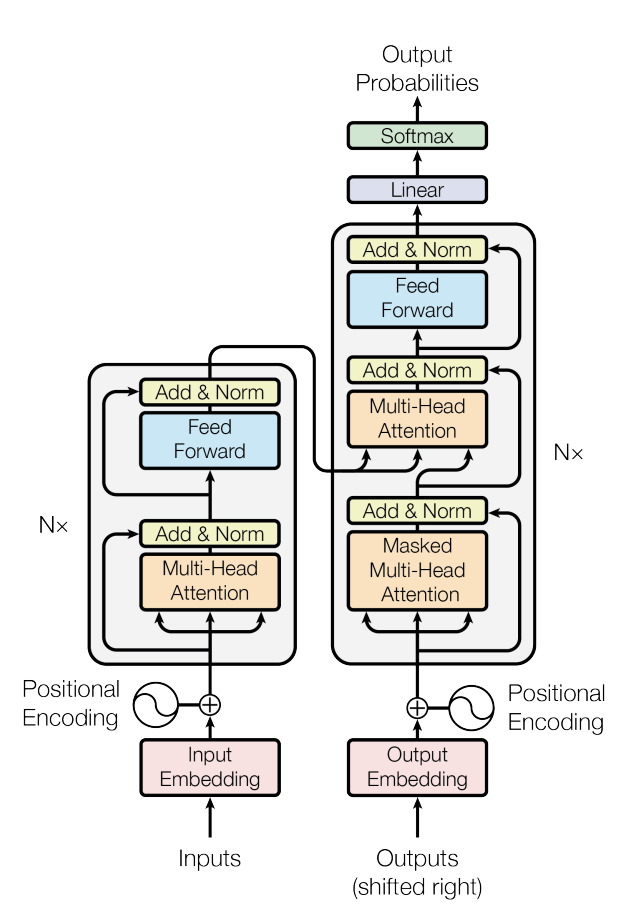
\includegraphics[width=\textwidth]{FIGS/transformer.png}
    \end{subfigure}
    % \begin{subfigure}[b]{0.65\textwidth}
    %     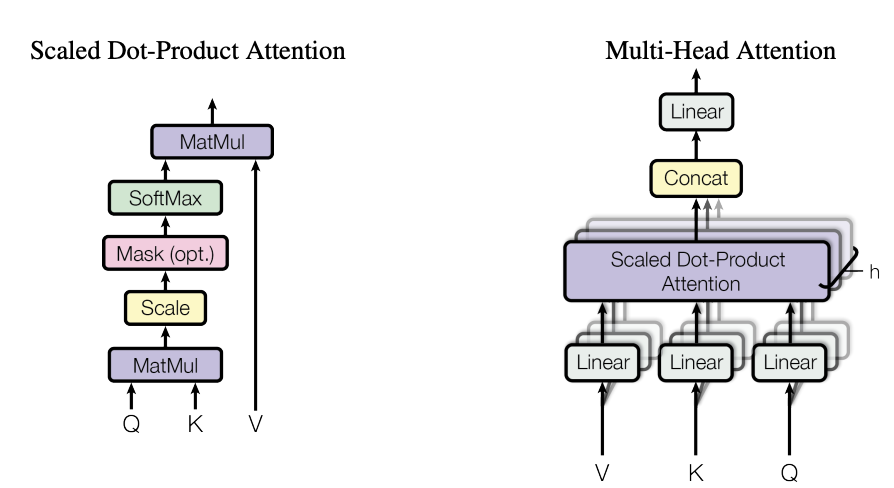
\includegraphics[width=\textwidth]{FIGS/multi-head.png}
    % \end{subfigure}
    \caption{Transformer architecture. Image credit: Vaswani \etal, 2017 \cite{vaswani2017attention}}
    \label{fig:transformer}
\end{figure}


Particular, BERT\cite{devlin2018bert} and Generative Pre-trained Transformer (GPT)~\cite{radford2019language} models are the two kinds of most popular Transformer-based model. 
One big distinction between them also lies in the attention module. The BERT employs the self-attention module that processes bidirectional representation, allowing reading text from left-to-right and right-to-left, while the GPT employs the masked self-attention module for unidirectional processing, as shown in Fig.~\ref{fig:bert2gpt}. Another difference is that the BERT uses the Transformer's encoder segment, while the GPT uses the decoder segment. 

\begin{figure}[!h]
    \centering
        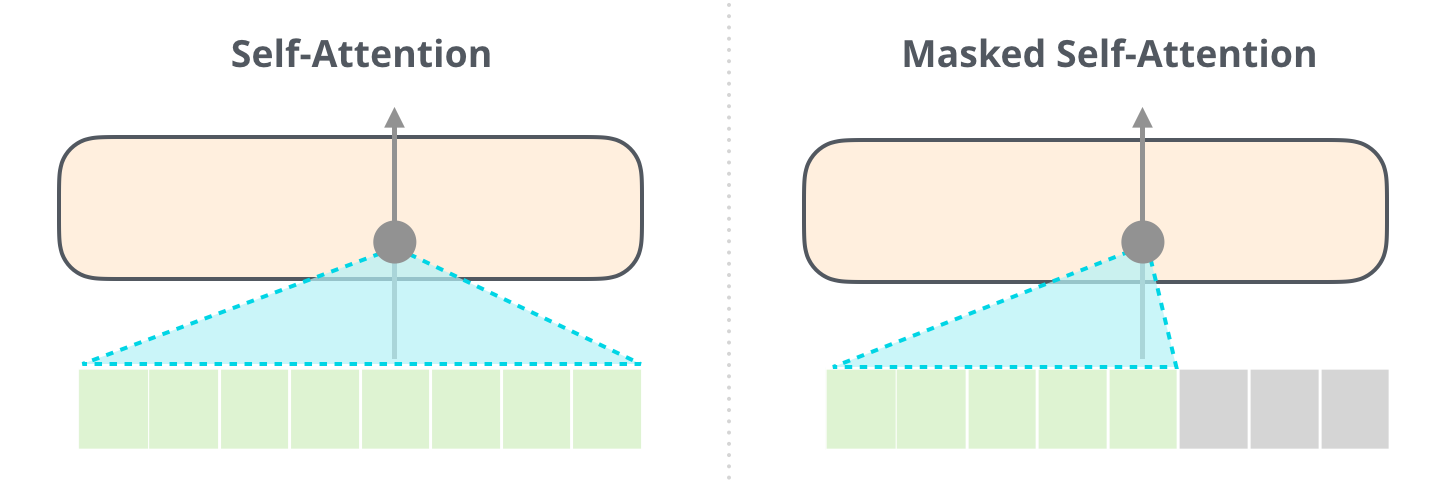
\includegraphics[width=0.8\textwidth]{FIGS/self-attention-and-masked-self-attention.png}
    \caption{Self-attention in BERT vs masked self-attention in GPT. Image credit: Jay Alammar \href{https://jalammar.github.io/illustrated-gpt2/}{https://jalammar.github.io/illustrated-gpt2/}}
    \label{fig:bert2gpt}
\end{figure}

Using attention gives us a way to see how the model attends to different parts of the input sentence, largely improving the model interpretability for decision making. 
Many tools have been developed to visualize the attention of the Transformer-based model. 
In this implementation, an open-source tool called BertViz~\cite{vig2019bertviz} was employed for model visualization from three perspectives: attention-head view, model view, and neuron view. 
A BERT and A GPT pre-trained model were investigated which were tested on the same sentence for comparison.


\section{Method}
\subsection{Model}
A BERT and A GPT model released in the \href{https://huggingface.co/models?sort=downloads&search=bert}{Hugging Face} model zoo were used:
\textbf{BERT}: ``bert-base-uncased";
\textbf{GPT-2}: ``gpt2''

\subsection{Testing data}
A sentence: \textit{``this bird cannot fly in the sky, because it is too heavy''}. In this sentence, ``it'' indicates the bird. 

\subsection{Attention head view}
\label{sec:head}
The attention-head view function provided by BertViz is to visualize the attention patterns produced by one or more attention heads in a given transformer layer. 
In this view, self-attention is represented as lines connecting the tokens that are attending (left) with the tokens being attended to (right). 
Colors represent the corresponding attention heads, while line weight reflects the attention score.

As shown in Fig~\ref{fig:head_view_gpt}, each head in the GPT-2 can produce a distinct attention pattern, since the attention heads do not share parameters. 
The top left figure shows all the tokens attend the first word ``this'' in the attention head of layer 7, while the head in the top right figure seems to generate attention dispersed evenly across previous
words.
The former pattern seems to be a null pattern that is produced when the linguistic property captured by the attention head doesn't appear in the input text. 
It would make the model more interpretable by disentangling the null attention from attention related to the first token.
The bottom two figures show the lexical pair patterns captured by the GPT-2. 
For example, $fly\leftrightarrow bird$ and $heavy\leftrightarrow bird$ show high attention, which correctly describes the relationship between behavior or characteristic and the entity.
Understanding this relationship might help the model understand the reasoning process that why the bird cannot fly. 

\begin{figure}[!h]
    \centering
    \begin{subfigure}[b]{0.48\textwidth}
        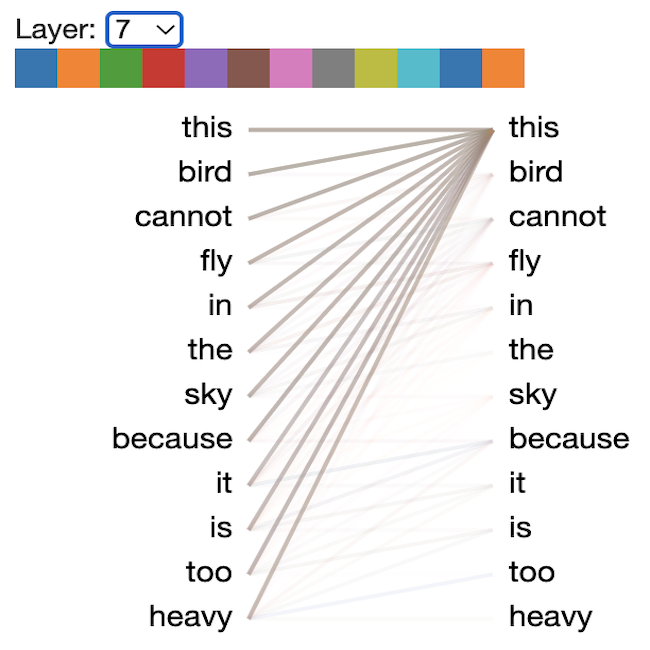
\includegraphics[width=\textwidth]{FIGS/gpt2_head_l7.png}
    \end{subfigure}
    \hfill
    \begin{subfigure}[b]{0.48\textwidth}
        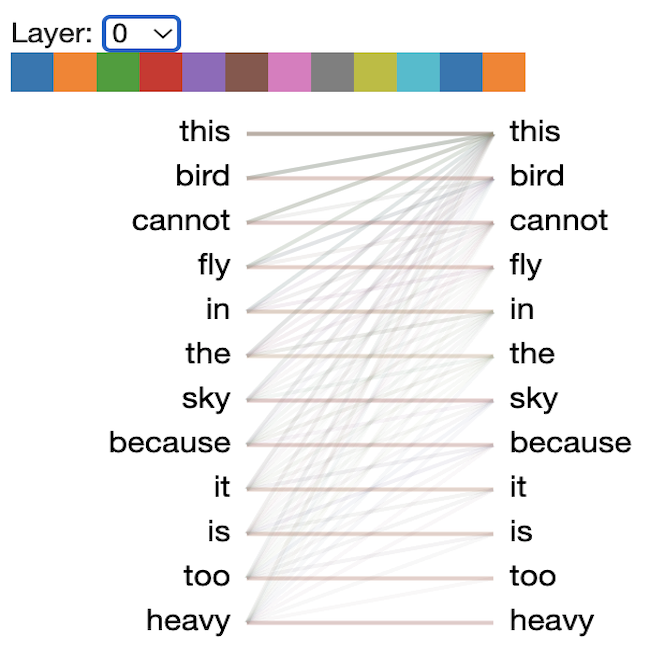
\includegraphics[width=\textwidth]{FIGS/gpt2_head_l0.png}
    \end{subfigure}
    \vfill
    \begin{subfigure}[b]{0.48\textwidth}
        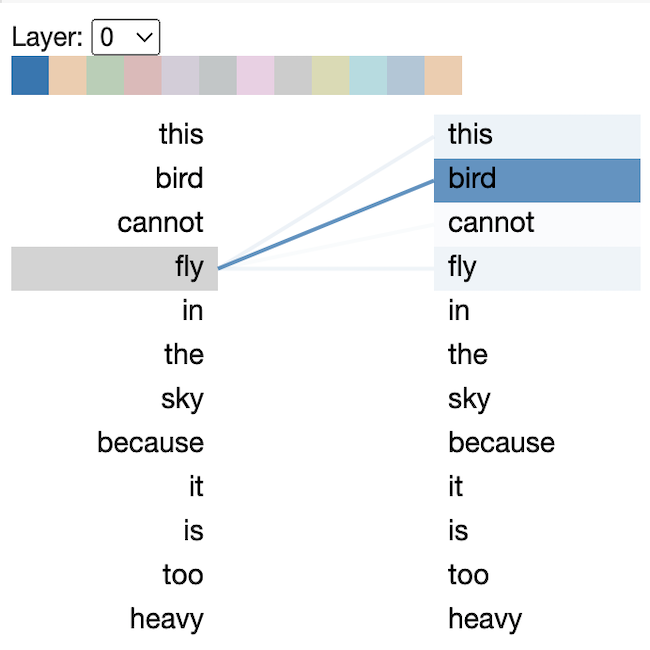
\includegraphics[width=\textwidth]{FIGS/gpt2_head_l0_fly.png}
    \end{subfigure}
    \hfill
    \begin{subfigure}[b]{0.48\textwidth}
        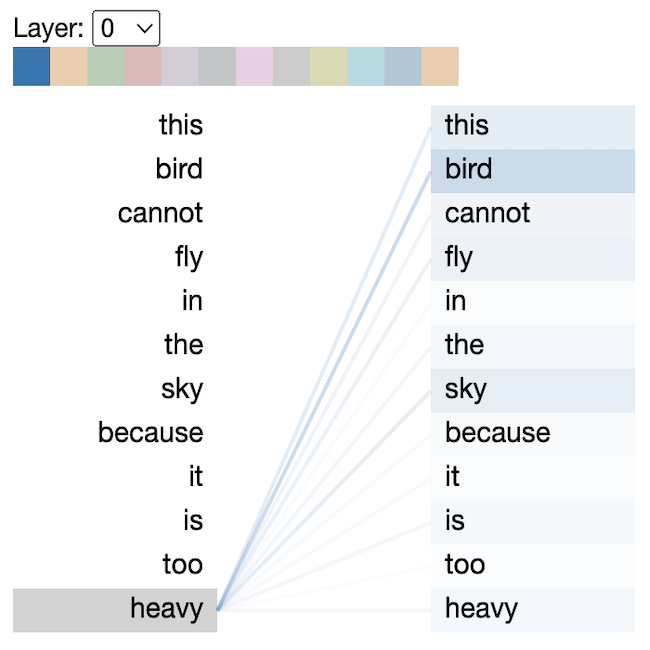
\includegraphics[width=\textwidth]{FIGS/gpt2_head_l0_heavy.png}
    \end{subfigure}
    \caption{Attention head view of GPT-2 on the sample text. Top left and right images represent the attention head of layer 7 and layer 0, respectively. 
    center figures represent different layers. 
    The bottom left and right images represent the attentions of tokens ``fly'' and ``heavy'' on the layer 0 ahd head 0.}
    \label{fig:head_view_gpt}
\end{figure}


For comparison, the head attentions in the BERT model were investigated, as shown in Fig~\ref{fig:head_view_bert}.
We can clearly see the difference between the unidirectional representation in GPT-2 and the bidirectional representation in BERT.
In addition, a delimiter-focused attention\cite{vig2019bertviz} pattern is observed in the top left figure, where most attention of tokens attend the sentence separator. Such a pattern means that an attention head can't find anything else in the input sentence to focus on, showing that BERT has designated a small set of neurons focusing on [SEP].
The bottom two figures show the bag-of-words attention pattern~\cite{vig2019bertviz}, where the attention is divided evenly across all words in the same sentence separated by the [SEP] token. 
It implies that the BERT might capture the sentence-specific meaning by focusing computing a bag-of-words embedding in the same sentence.
All these results showed the distinct attention patterns acquired by the GPT-2 and BERT.

\begin{figure}[!h]
    \centering
    \begin{subfigure}[b]{0.48\textwidth}
        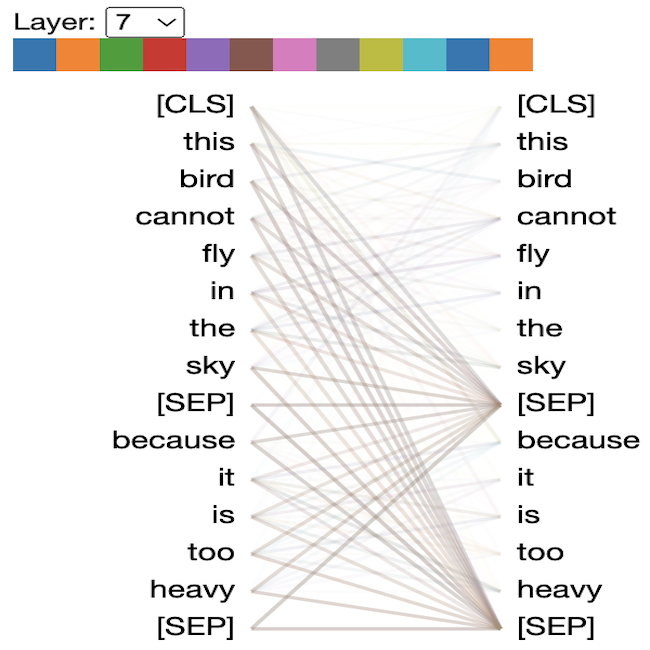
\includegraphics[width=\textwidth]{FIGS/bert_head_l7.png}
    \end{subfigure} 
    \hfill
    \begin{subfigure}[b]{0.48\textwidth}
        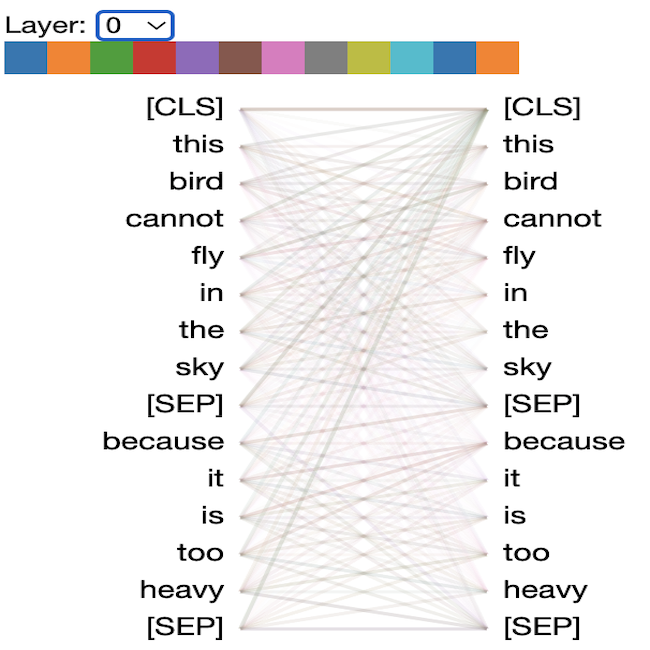
\includegraphics[width=\textwidth]{FIGS/bert_head_l0.png}
    \end{subfigure}
    \vfill
    \begin{subfigure}[b]{0.48\textwidth}
        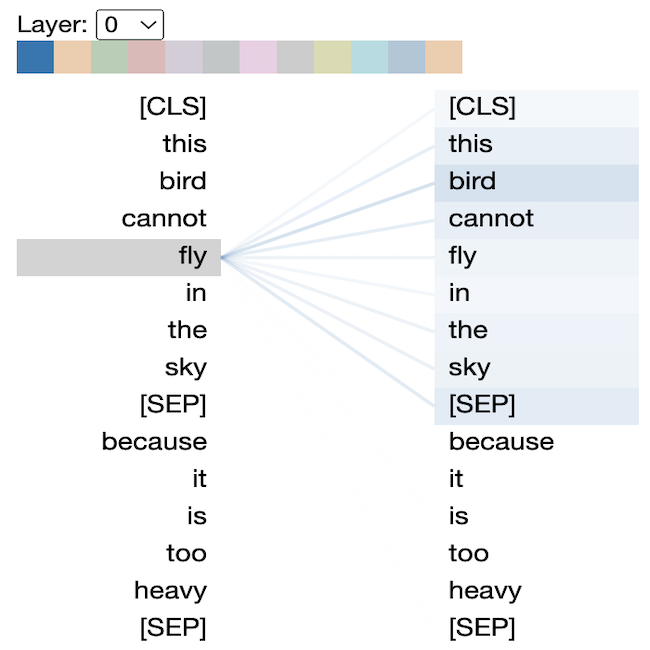
\includegraphics[width=\textwidth]{FIGS/bert_head_l0_fly.png}
    \end{subfigure}
    \hfill
    \begin{subfigure}[b]{0.48\textwidth}
        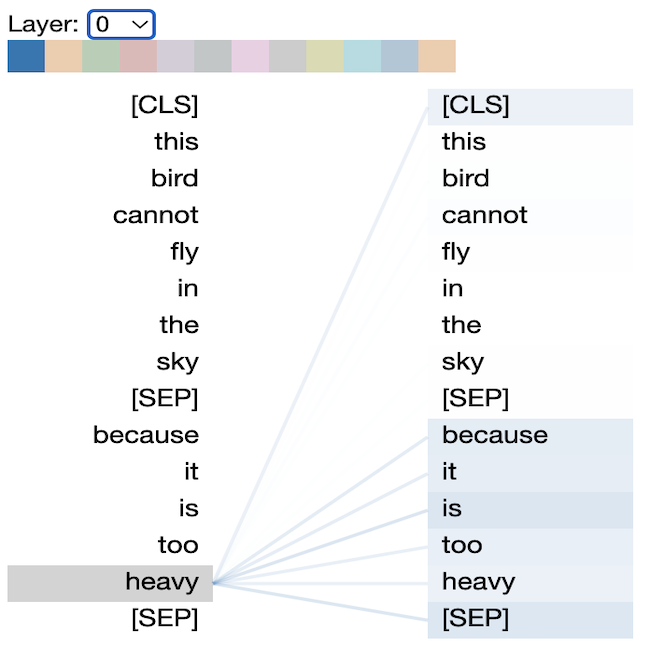
\includegraphics[width=\textwidth]{FIGS/bert_head_l0_heavy.png}
    \end{subfigure} 
    \caption{Attention head view of BERT on the sample text. Each figure corresponds to those of GPT-2's. [SEP] means the sentence separator; [CLS] means the beginning of the sentence.}
    \label{fig:head_view_bert}
\end{figure}

\subsection{Model view}
\label{sec:model}
The model view provides a bird's-eye view of attention across all of the layers and heads of the model for a particular input, as shown in Fig.~\ref{fig:model_view}.
It enables us to check the attention heads across all layers and see how attention patterns evolve throughout the model. 
For example, we can observe that each token seems to focus on the same token (layer 0, head 1) or on the previous token (layer 1, head 0).
Similar patterns described in the section ~\ref{sec:head} are easily identified, like delimiter-focused attention (layer 3, head 0) and bag-of-words attention (layer0, head 0). 

\begin{figure}[!h]
    \centering
    \begin{subfigure}[b]{0.8\textwidth}
        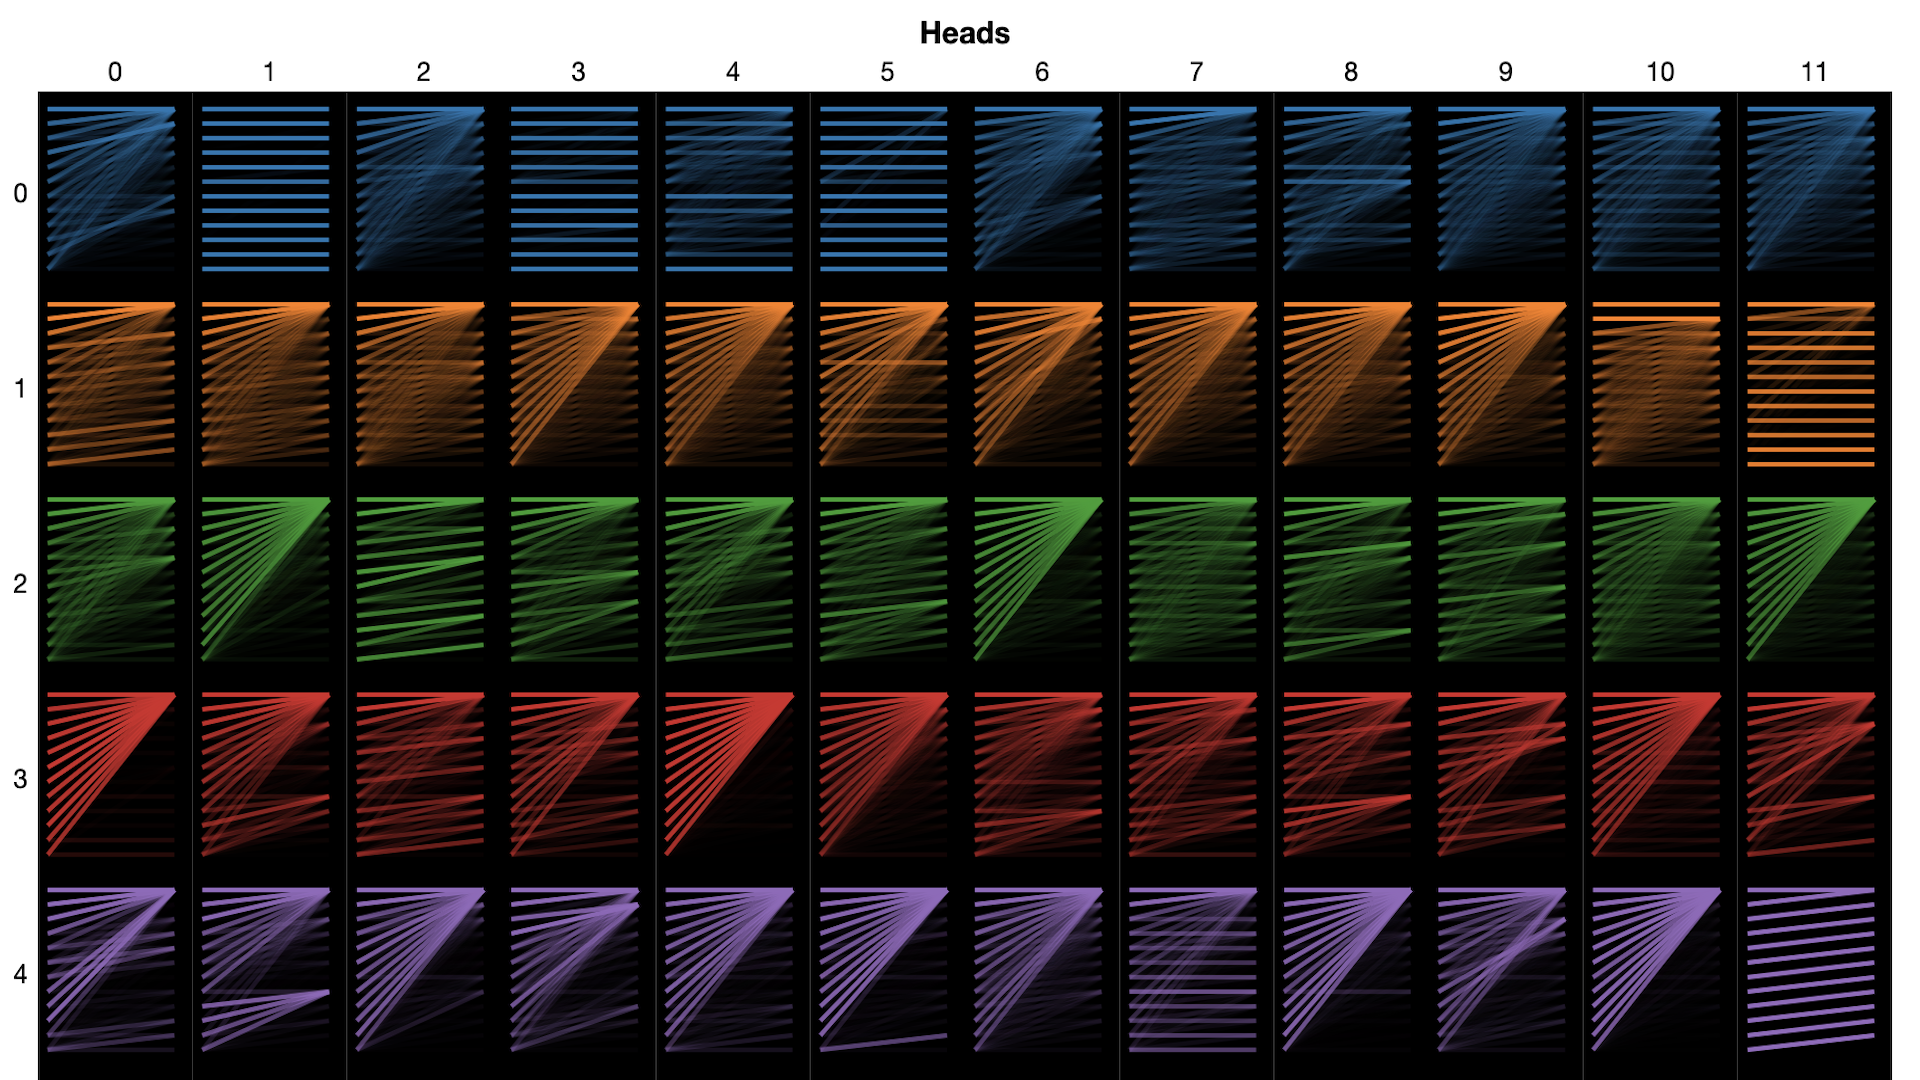
\includegraphics[width=\textwidth]{FIGS/gpt2_model.png}
        \caption{GPT-2}
    \end{subfigure} 
    \hfill
    \begin{subfigure}[b]{0.8\textwidth}
        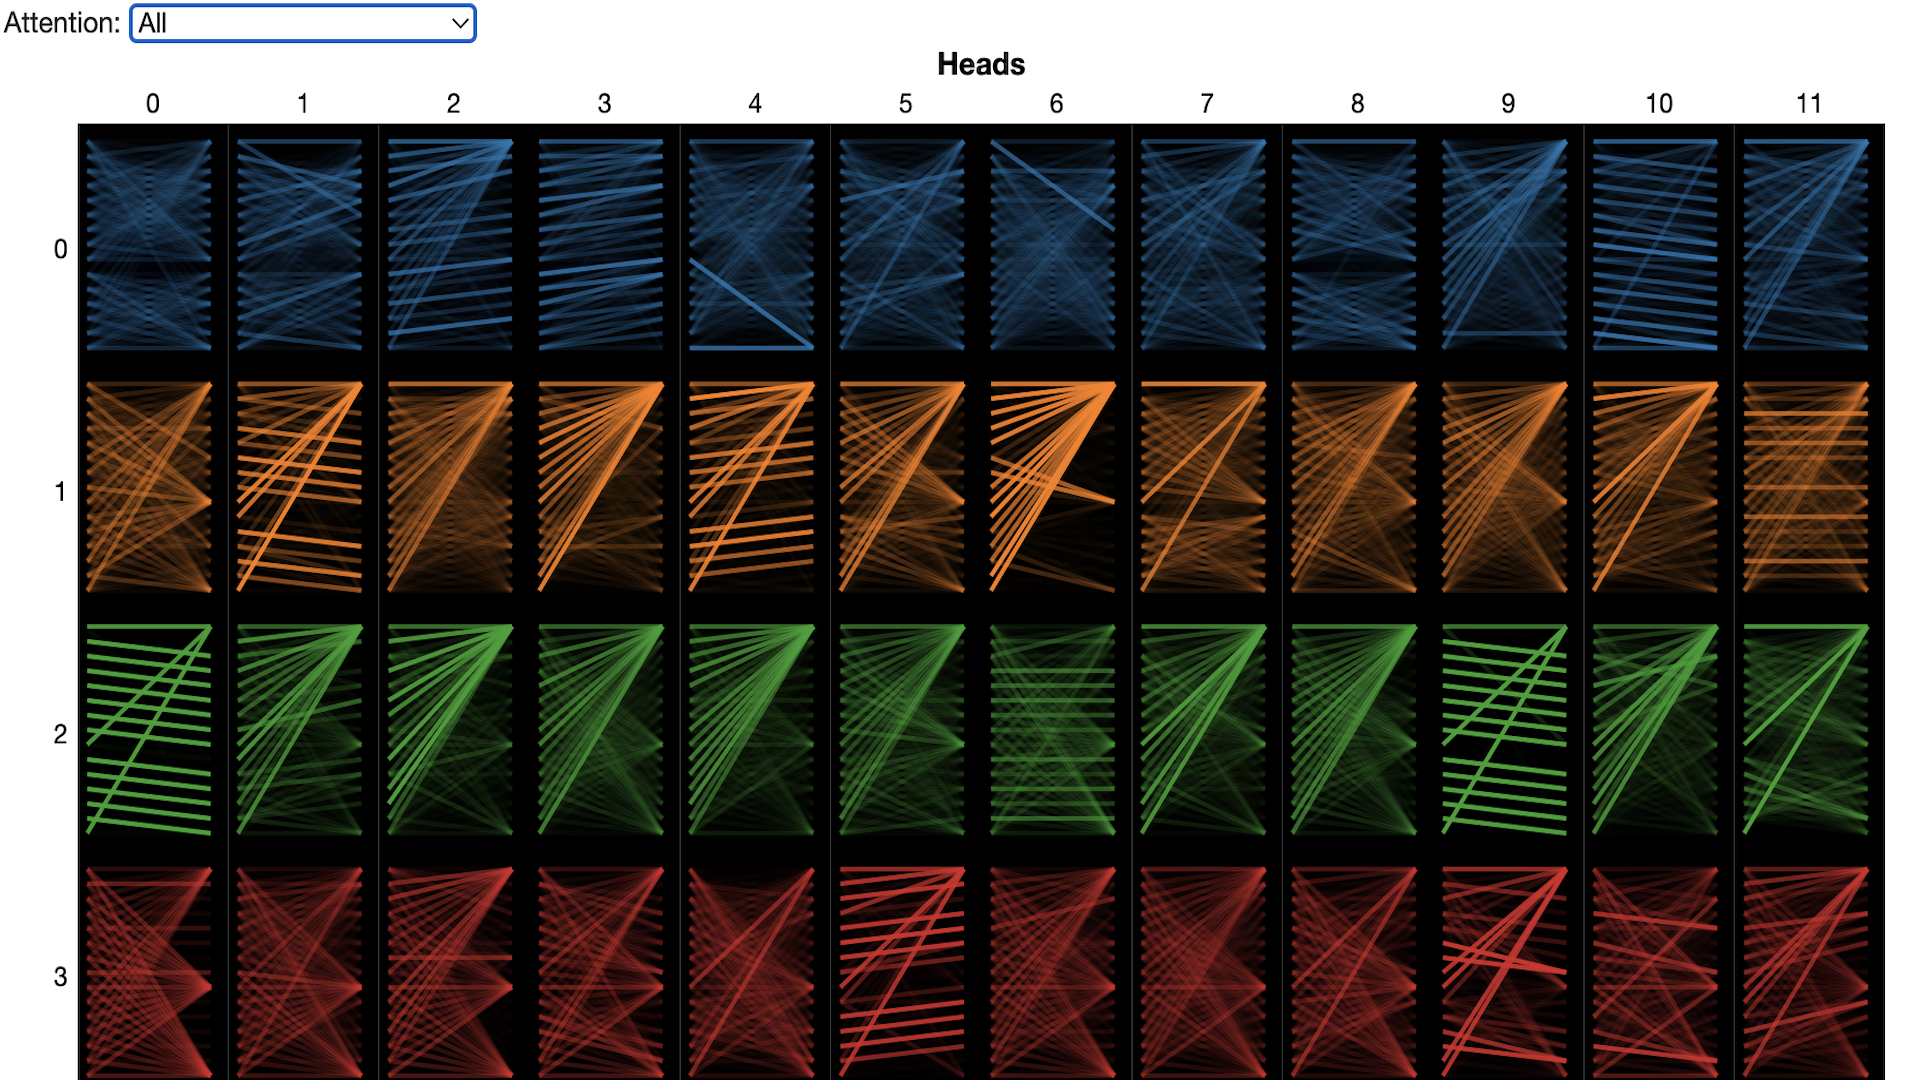
\includegraphics[width=\textwidth]{FIGS/bert_model.png}
        \caption{BERT}
    \end{subfigure}
    \vfill
    \caption{Model view samples of GPT-2 and BERT, showing first 4 layers and all 12 heads. Attention heads are presented in a Tabular form, where rows represents the layers and columns represent the heads.}
    \label{fig:model_view}
\end{figure}

Of course, the attention head of a specific layer and head could be enlarged for checking the detailed tokens, as shown in Fig.~\ref{fig:model_view_detail}. The similar patterns discussed above can be observed.

\begin{figure}[!h]
    \centering
    \begin{subfigure}[b]{0.32\textwidth}
        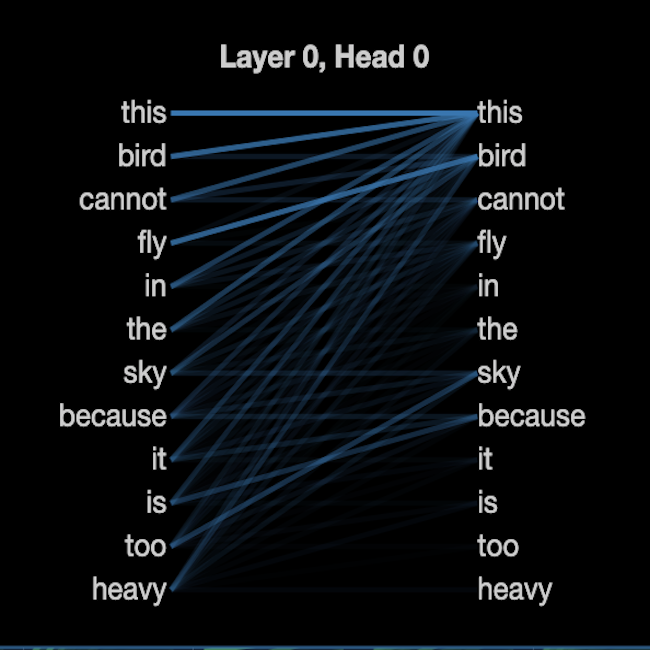
\includegraphics[width=\textwidth]{FIGS/gpt2_model_L0H0.png}
        % \caption{}
    \end{subfigure}
    \hfill
    \begin{subfigure}[b]{0.32\textwidth}
        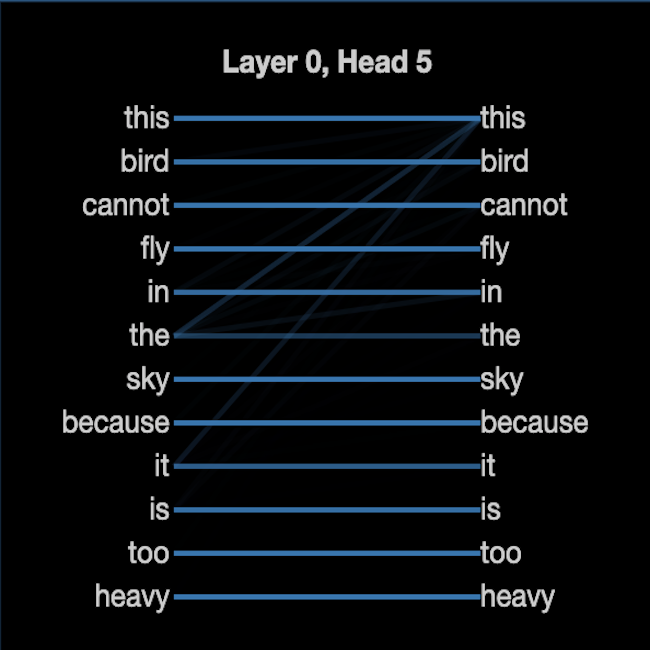
\includegraphics[width=\textwidth]{FIGS/gpt2_model_L0H5.png}
        % \caption{GPT-2}
    \end{subfigure}
    \hfill
    \begin{subfigure}[b]{0.32\textwidth}
        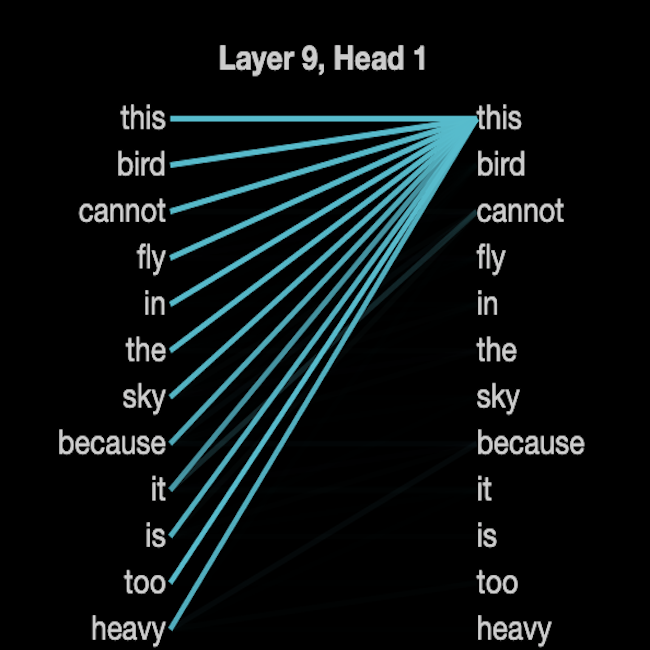
\includegraphics[width=\textwidth]{FIGS/gpt2_model_L9H1.png}
        % \caption{}
    \end{subfigure}
    \vfill
    \begin{subfigure}[b]{0.32\textwidth}
        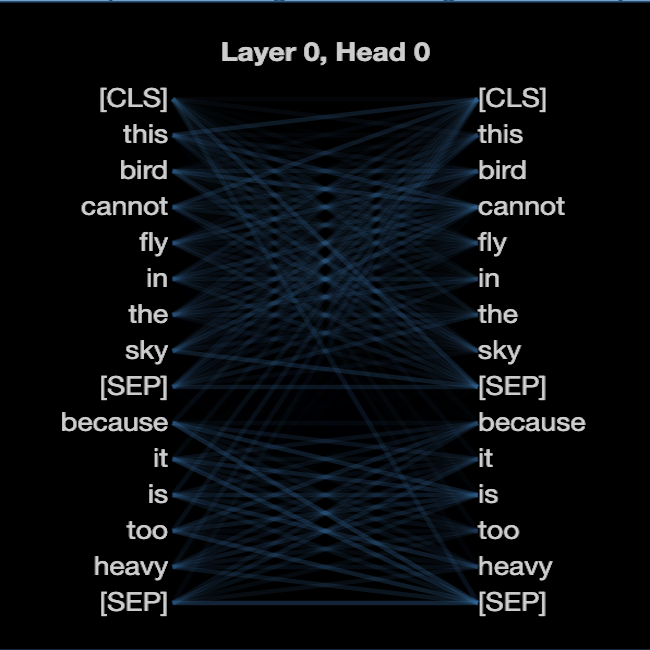
\includegraphics[width=\textwidth]{FIGS/bert_model_L0H0.png}
        % \caption{}
    \end{subfigure}
    \hfill
    \begin{subfigure}[b]{0.32\textwidth}
        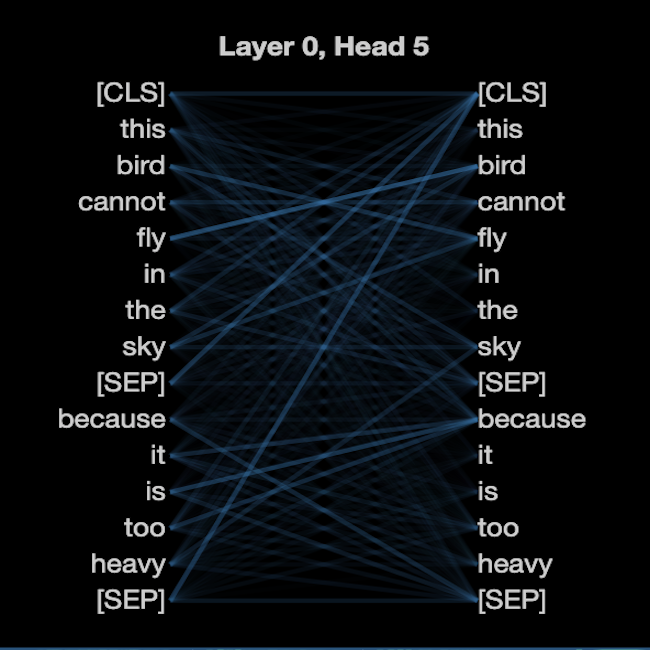
\includegraphics[width=\textwidth]{FIGS/bert_model_L0H5.png}
        % \caption{BERT}
    \end{subfigure}
    \hfill
        \begin{subfigure}[b]{0.32\textwidth}
            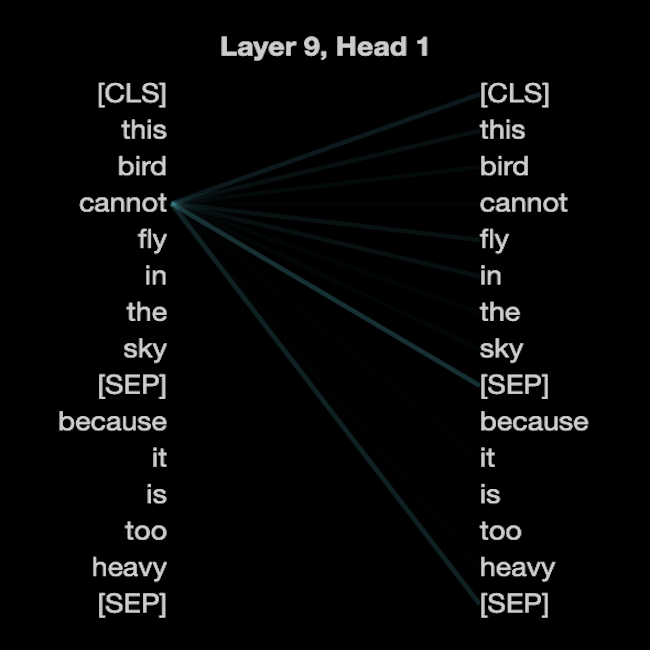
\includegraphics[width=\textwidth]{FIGS/bert_model_L9H1.png}
            % \caption{}
    \end{subfigure}
    \caption{Attention head view particular layer and head of GPT-2 (top row) and BERT (bottom row) in the model view.}
    \label{fig:model_view_detail}
\end{figure}

\subsection{Neuron view}
\label{sec:neuron}
The neuron view visualizes the individual neurons in the query and key vectors and shows how they interact to produce attention scores, providing the internal explanation of a particular attention head and showing how BERT forms these patterns.
Given a selected token, it traces the computation of attention from that token to the other tokens in the sequence.
The element-wise product of the vectors shows how individual neurons contribute to the attention
The token ``heavy'' and ``fly'' discussed above are also visualized in Fig.~\ref{fig:neuron}. 
For example, the bottom left figure shows a bag-of-words attention pattern, where the element-wise products are positive for tokens in the same sentence and negative for tokens in different sentences. 
The reason is that the corresponding query
and key neurons have high-magnitude values of the same sign for tokens in the same sentence, but of
opposite sign for tokens in the opposite sentence. 
When specific neurons are linked to a tangible outcome, it implies that human intervention might be introduced into the model to alter the values of the relevant neurons, showing the benefit of model interpretability. 


\begin{figure}[!h]
    \centering
    \begin{subfigure}[b]{0.48\textwidth}
        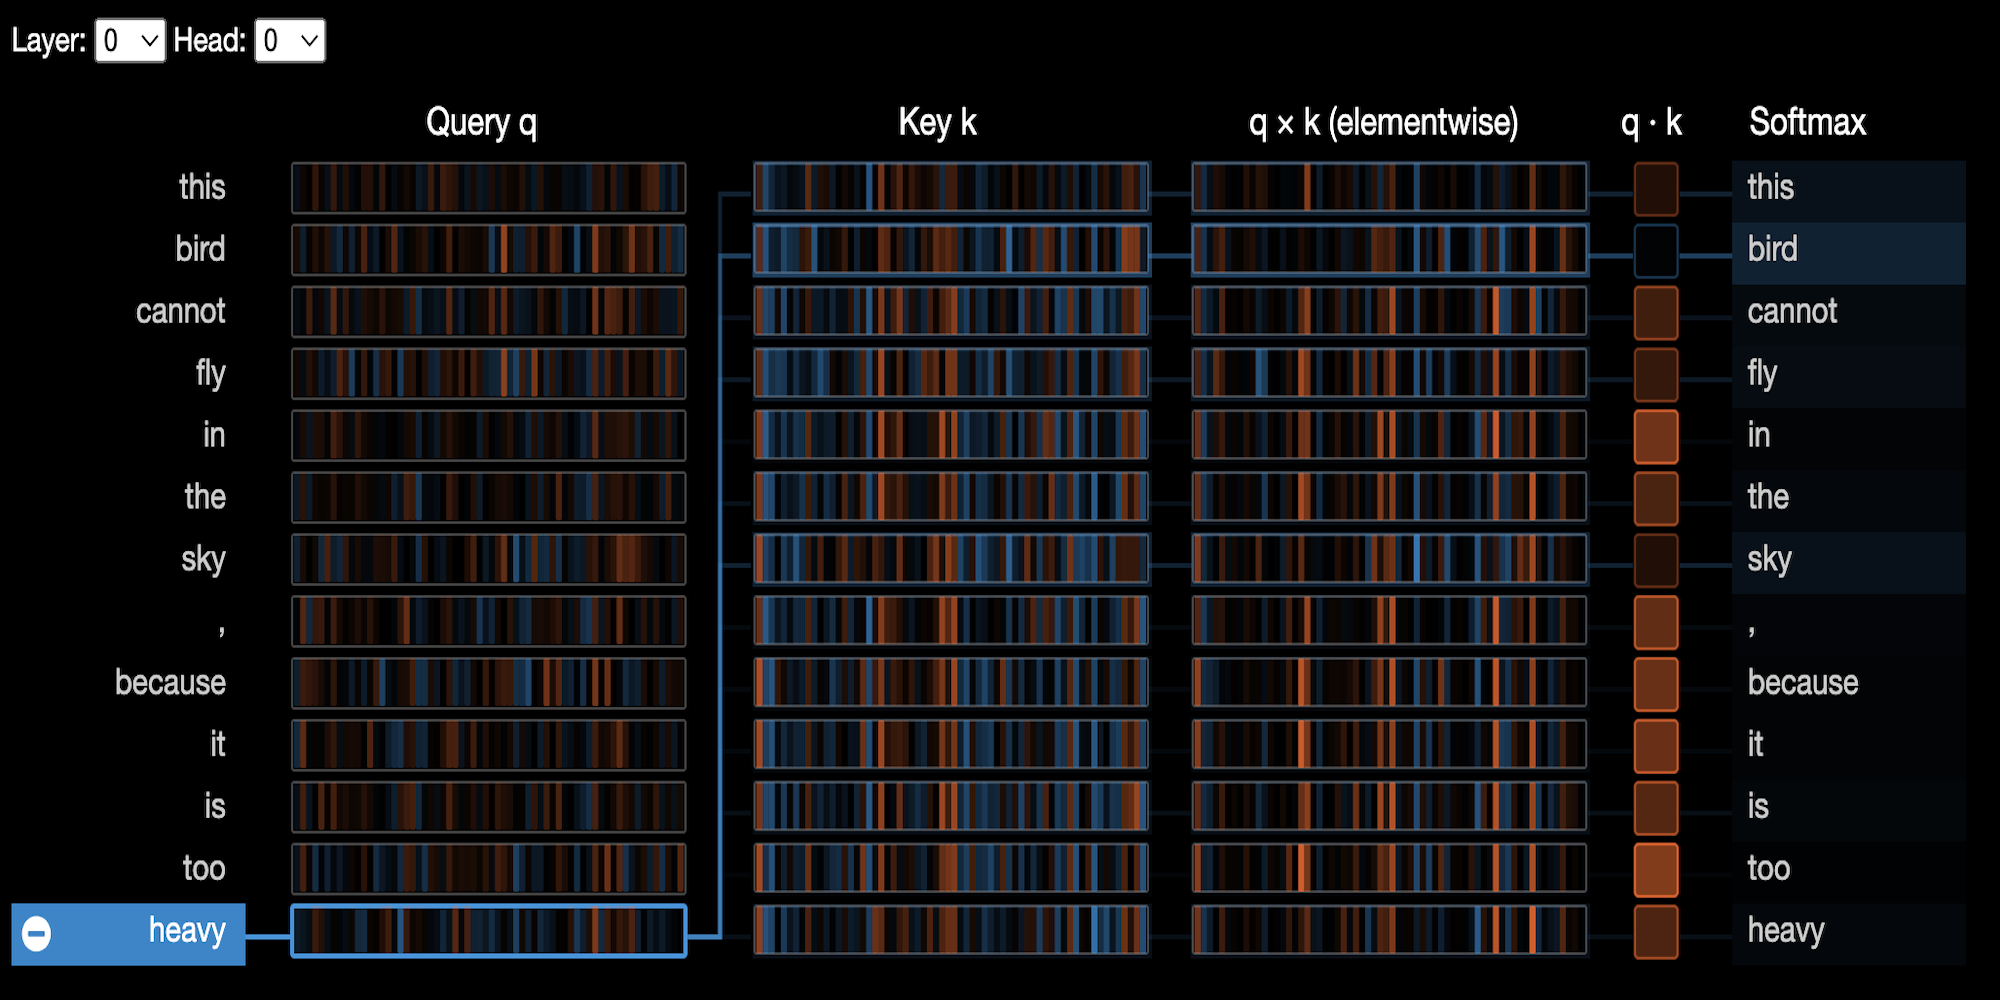
\includegraphics[width=\textwidth]{FIGS/gpt2_neuron_L0H0_heavy.png}
    \end{subfigure} 
    \hfill
    \begin{subfigure}[b]{0.48\textwidth}
        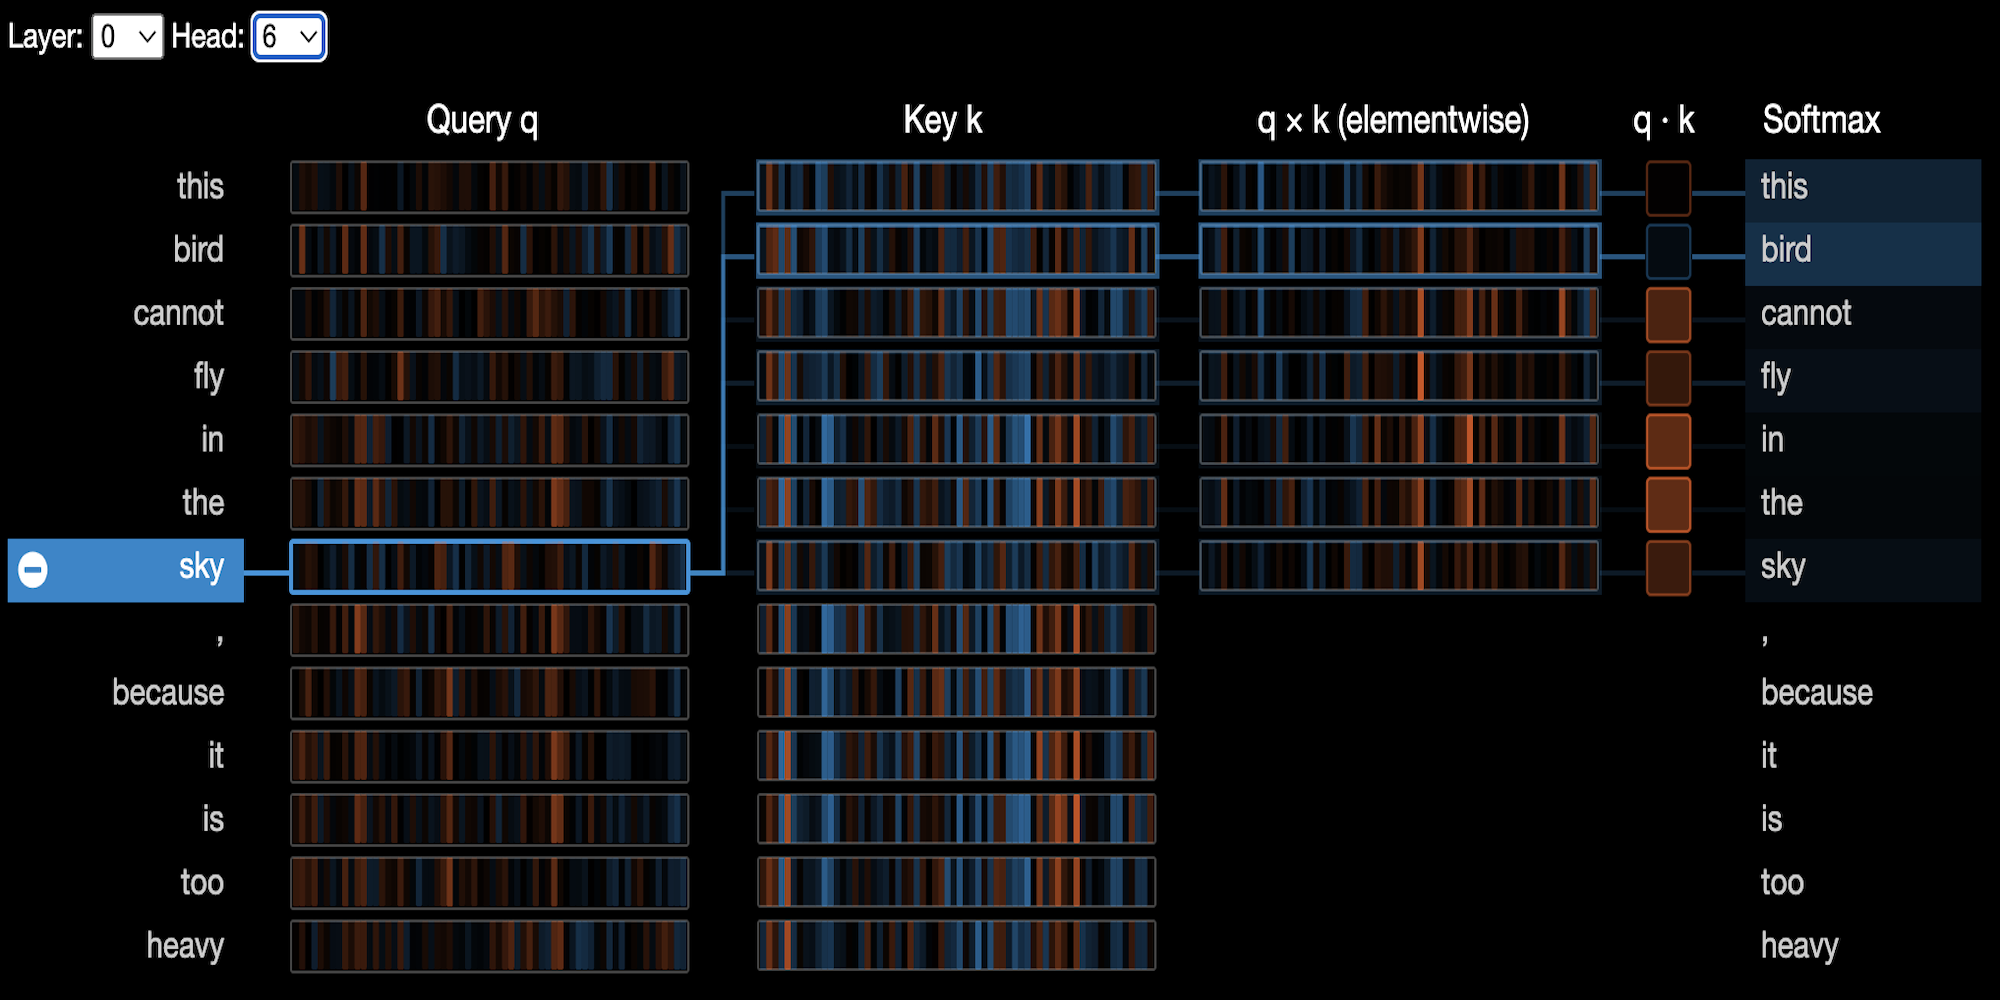
\includegraphics[width=\textwidth]{FIGS/gpt2_neuron_L0H6_sky.png}
    \end{subfigure}
    \vfill
    \begin{subfigure}[b]{0.48\textwidth}
        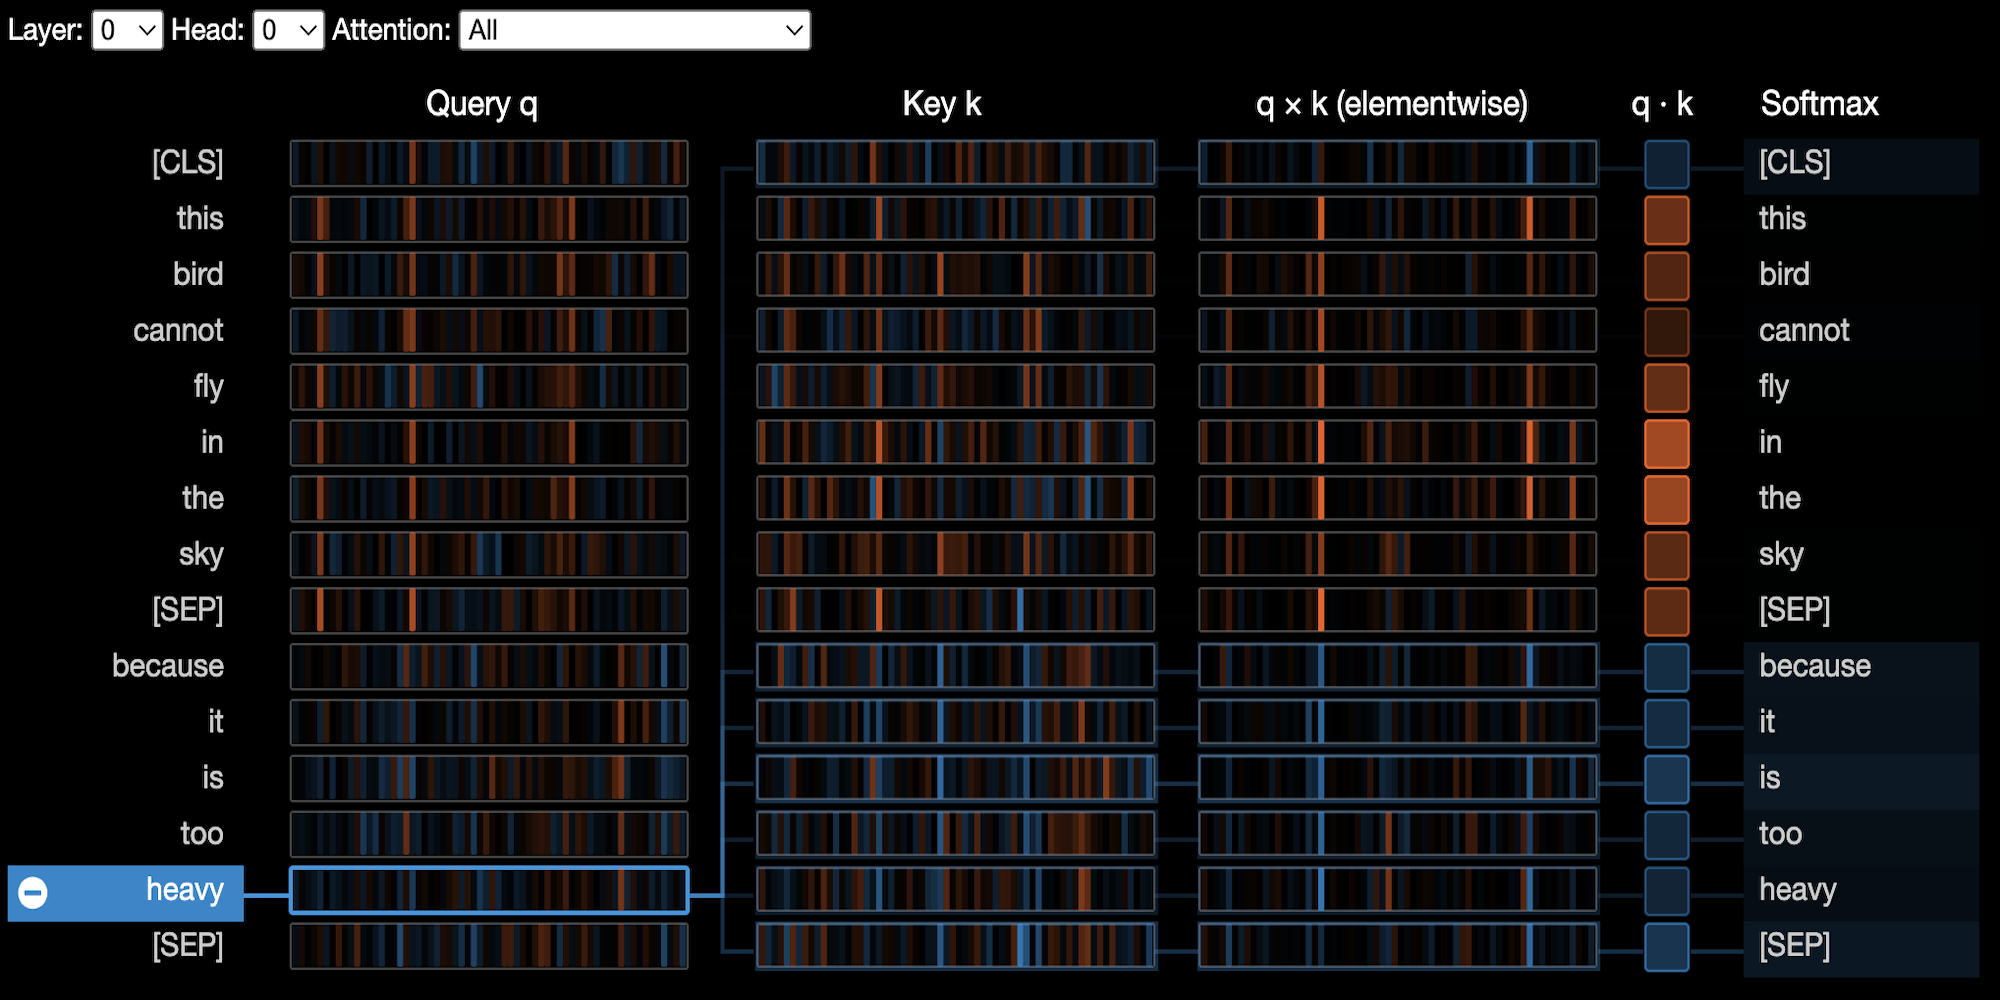
\includegraphics[width=\textwidth]{FIGS/bert_neuron_L0H0_heavy.png}
    \end{subfigure} 
    \hfill
    \begin{subfigure}[b]{0.48\textwidth}
        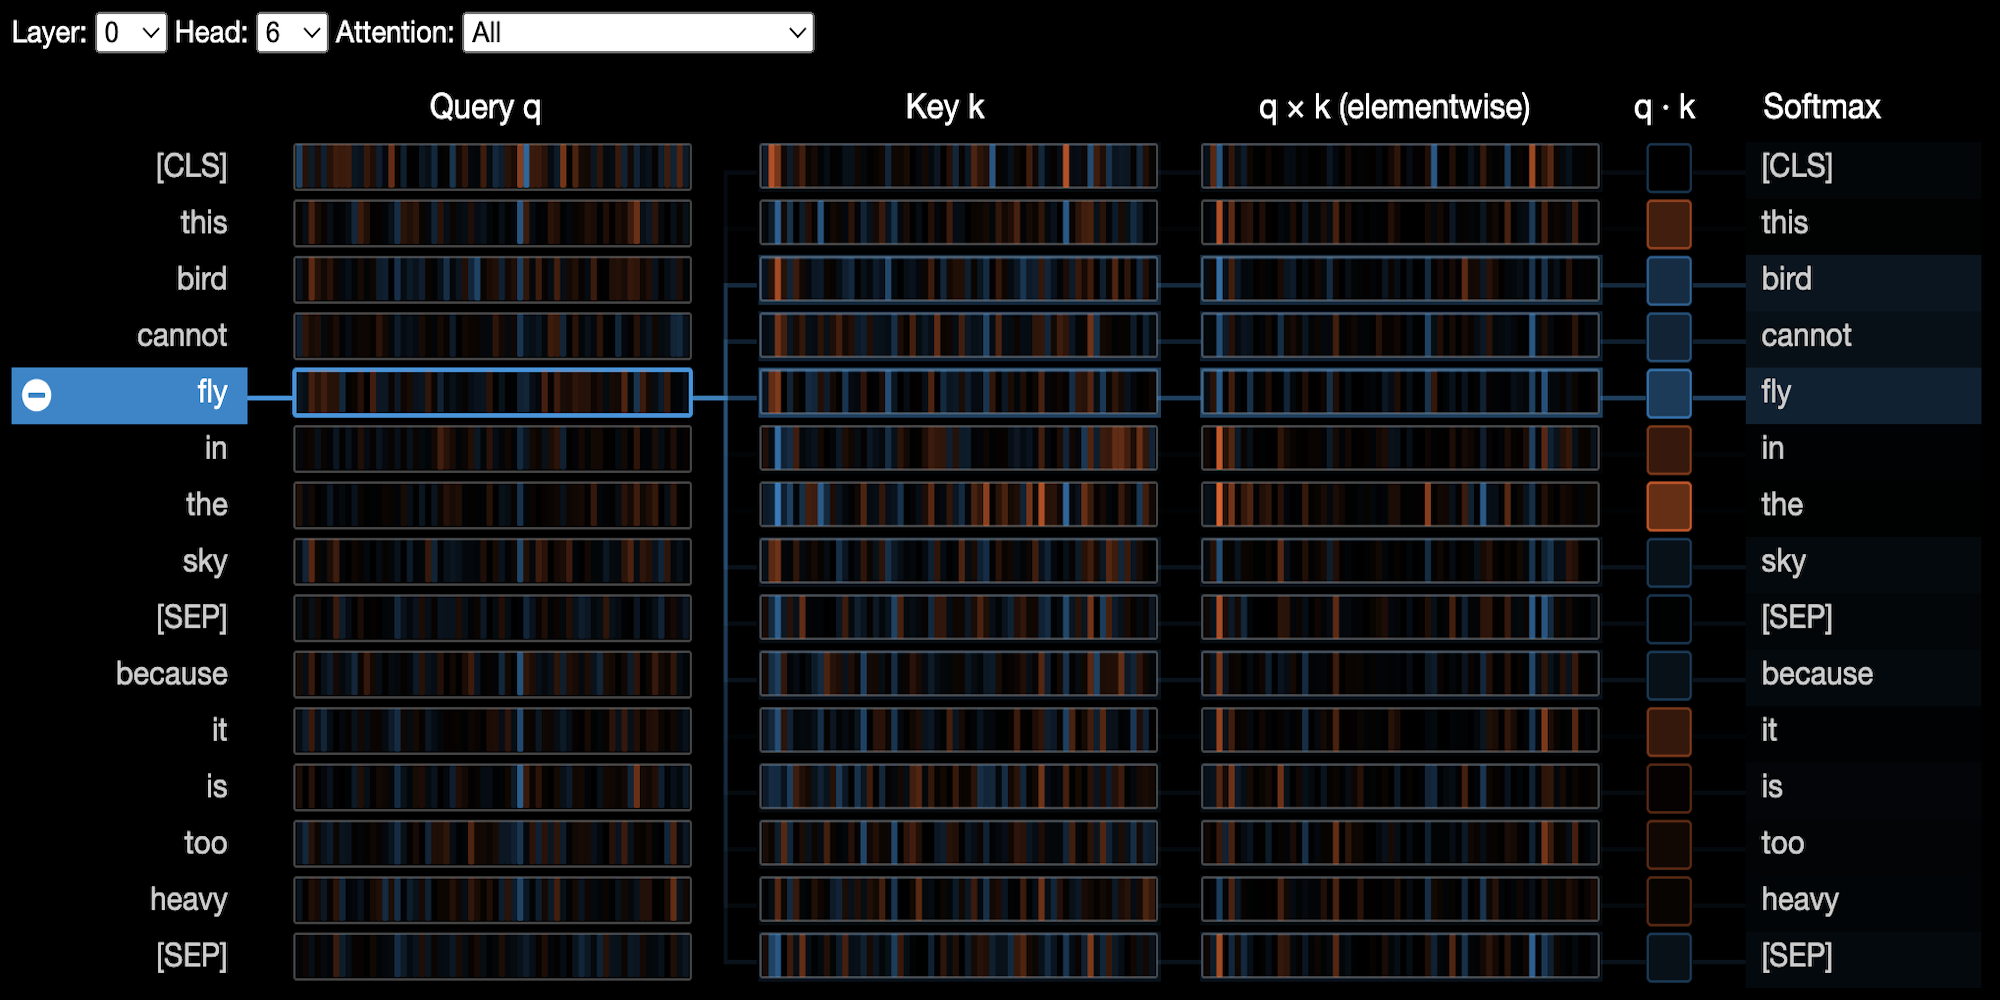
\includegraphics[width=\textwidth]{FIGS/bert_neuron_L0H6_fly.png}
    \end{subfigure}
    \caption{Neuron view examples of GPT-2 (top row) and BERT (bottom row). Query q: The 64-element query vector of the selected token paying attention; 
    Key k: The 64-element key vector of each token receiving attention;
    $q\times k$ (element-wise): The element-wise product of the selected token's query vector and each key vector;
    $q\dot k$: The dot product of the selected token's query vector and each key vector;
    Softmax: The softmax of the scaled dot-product from previous column. This equals the attention received by the corresponding token.
    Positive and negative values are colored blue and orange, respectively, with color saturation showing the value magnitude.}
    \label{fig:neuron}
\end{figure}


\section{Conclusion}
In this implementation, we employed the BertViz tool for visualizing attention in Transformer-based language models. By analyzing a sample text sentence on both BERT and GPT-2, we found attention visualization could provide insights into how the language models try to understand the sentence. 
In this way, hacking into the language model could give us better model interpretability and potential controllability. 


\vspace{-0.2cm}
\scriptsize{
\bibliographystyle{abbrv}
\bibliography{LECTURE_EXPLAINABILITY_I_IMPLEMENTATION_SP22}
}

\end{document} 